\documentclass{beamer}
\mode<presentation>
\usetheme{inf}
\usepackage[math]{kurier}
\usepackage{fmtcount}
\usepackage{tikz}
\usepackage[europeanresistors]{circuitikz}
\usetikzlibrary{shapes,arrows}
\usepackage{mapdefs}
\usepackage{xmission}
\definecolor{hubsblue}{RGB}{2,72,142}
\def\HUBS{{\color{hubsblue}HUBS }}

\begin{document}
\title{Update: Community Networking in Scotland}
\author{William Waites\\\url{ww@hubs.net.uk}}
%\lfcs
\institute{{\large \HUBS \textsc{c.i.c.}} \and 
  \&\hspace{5pt}%
  \begin{minipage}{0.3\textwidth}
    \begin{center}
      School of Informatics\\University of Edinburgh
    \end{center}
  \end{minipage}
}
\projectlogo{\includegraphics[height=0.07\paperheight]{hubs-logo}}

\setbeamertemplate{headline}{}

\date[IXS]{IX Scotland Meeting, Edinburgh\\December 1\fmtord{st}, 2014}
{
    \begin{frame}
      \titlepage
    \end{frame}
}
\begin{frame}
  \frametitle{Setting}
  \begin{tikzpicture}[overlay]
    \europe
  \end{tikzpicture}
\end{frame}
\begin{frame}
  \frametitle{Setting}
  \begin{tikzpicture}[overlay]
    \europe\scotland
  \end{tikzpicture}
\end{frame}
\begin{frame}
  \frametitle{Setting}
  \begin{tikzpicture}[overlay]
    \europe\scotland\wcn
  \end{tikzpicture}
\end{frame}
\begin{frame}
  \frametitle{Setting}
  \begin{tikzpicture}[overlay]
    \europe\scotland\wcn\arnisdale
  \end{tikzpicture}
\end{frame}
\begin{frame}
  \begin{tikzpicture}[overlay]
    \node at (5.5, -0.5) {%
      \includegraphics[width=1.05\paperwidth]{Cview.jpg}%
    };%
    \node (arnisdale) at (10,-2) {\Large \color{hubsblue} Arnisdale};
    \node (corran) at (9,0) {\Large \color{hubsblue} Corran};
    \draw[arrows=-triangle 45, color=hubsblue] (arnisdale) to (6.75,-2.75);
    \draw[arrows=-triangle 45, color=hubsblue] (corran) to (5,0.75);
  \end{tikzpicture}
\end{frame}
\begin{frame}
  \frametitle{Arnisdale}
  \begin{columns}
    \column{0.3\textwidth}
    \begin{center}
      \vspace{-2\baselineskip}
      \includegraphics[width=1.2\textwidth]{starting.jpg}\\
      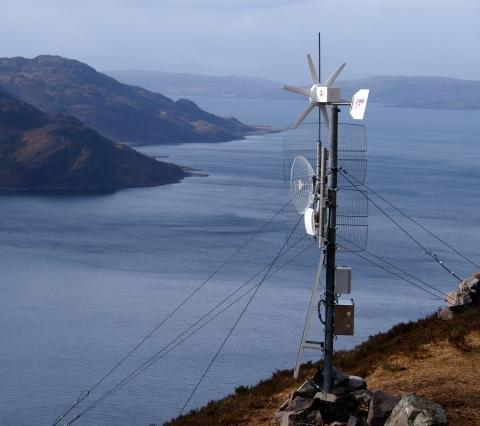
\includegraphics[width=1.2\textwidth]{stick.jpg}
    \end{center}
    \column{0.7\textwidth}
    \begin{itemize}%[<+->]
      \item 9 miles $=$ 15km from the telephone exchange at Glenelg
      \item Copper wire barely good enough for 2400 baud\\
        $\ldots$ Nevermind *DSL
      \item Anyways, Glenelg only has maybe a couple of E1s
      \item Ladhar Bheinn blocks satellites (\& slow \& expensive)
      \item Residents wrote many letters to BT, politicians\\
        $\ldots$ to no avail
      \item Eventually decided to build a network themselves
    \end{itemize}
  \end{columns}
\end{frame}
\begin{frame}
  \frametitle{Tegola\footnote{An Italian word meaning \textit{tile},
      this name is in honour of the effect of wet roof tiles on 2.4GHz
      RF propagation which beset some early experiments.}}
  \begin{columns}
    \column{0.6\textwidth}
    \begin{itemize}
      \item Tegola -- Loch Hourn from 2008.
      \item Trial link from Corran 15km to Isleornsay sharing
        512kbps ADSL.
      \item Expanded to a ring of six masts
      \item Gateworkx, OpenWRT, Quagga, OSPF, 802.11a
      \item Giacomo Bernardi, Peter Buneman, Mahesh Marina (UoE)
      \item Upstream bandwidth from UHI Sabhal M\`{o}r Ostaig
    \end{itemize}
    \column{0.4\textwidth}
    \hspace{-2em}
    \includegraphics[width=1.1\textwidth]{mhialairigh-from-behind.jpg}
  \end{columns}
\end{frame}
\begin{frame}{The Neighbours}
  \begin{columns}
    \column{0.4\textwidth}
    \includegraphics[width=\textwidth]{corran-testing.jpg}\\
    \includegraphics[width=\textwidth]{inver-mast.jpg}\\
    \column{0.6\textwidth}
    \begin{itemize}
      \item Nearby islands \alert{Eigg}, and \alert{Rum} build
        networks on a similar model with advice from Tegola.
      \item \alert{Knoydart} in the next Loch builds theirs with help
        from Eigg.
      \item Later, \alert{Applecross} to the north joins in$\ldots$\\
        $\ldots$ and \alert{Locheil}\\
        $\ldots$ and northern \alert{Mull}\\
        $\ldots$ and \alert{Sleat}
      \item Farther afield \alert{Laggan}, \alert{Lothian},
        \alert{Heriot}, \alert {Stobo} and
        others$\ldots$
    \end{itemize}
  \end{columns}
\end{frame}
\begin{frame}
  \frametitle{Many Architectures}
  \begin{columns}
    \column{0.6\textwidth}
    \begin{itemize}
      \item \alert{\textsc{Not}} centrally managed
      \item Local networks built according to local skills --
        \emph{very} important
      \item Aversion to dynamic routing\\
        $\ldots$ but we \alert{want} redundant paths\\
        $\ldots$ more important for remote places -- (\textsc{mttr},
        no mobile coverage)
      \item Vendor firmware is limited
      \item OpenWRT too high a barrier
      \item ``serious'' routers too expensive\\
        $\ldots$ also too power hungry
    \end{itemize}
    \column{0.4\textwidth}
    \hspace{1em}\scalebox{0.8}{
      
\begin{tikzpicture}[overlay]
        \node[draw, ellipse, fill=cyan!20] at (1,2) { OLSR };
        \node[draw, ellipse, fill=blue!20] at (0.75,1) { \textsc{b.a.t.m.a.n}};
        \node[draw, ellipse, align=center, fill=blue!20] at (3.5,1.5) {
          \textsc{b.a.t.m.a.n} \\ $+$ PPPoE?};
        \node[draw, ellipse, align=center, fill=green!20] at (2.5, 0) { OSPF $+$ \\ PPPoE };
        \node[draw, ellipse, fill=green!20] at (0,0) { OSPF };
        \node[draw, ellipse, align=center, fill=orange!20] at (1,-1.5) { Static \\ Routing };
        \node[draw, ellipse, align=center, fill=orange!20] at (3.5,-1.5) { Flat $+$ \\ PPPoE };
        \node[draw, ellipse, align=center, fill=red!20] at (0,-3.5) { Flat $+$\\ Bridged };
        \node[draw, ellipse, align=center, fill=red!20] at (2.5,-3) { Telescope\\ NAT };
      \end{tikzpicture}
    }
  \end{columns}
\end{frame}
\begin{frame}{The Internet in Microcosm}
  \begin{columns}
    \column{0.3\textwidth}
    \begin{center}
      \vspace{-1\baselineskip}%
      \hspace{1em}\scalebox{1.3}{
        \begin{tikzpicture}[overlay]
          \begin{scope}
            \clip (-1.6,-2.25) rectangle (1.6,2.2);
            \node at (0,0) {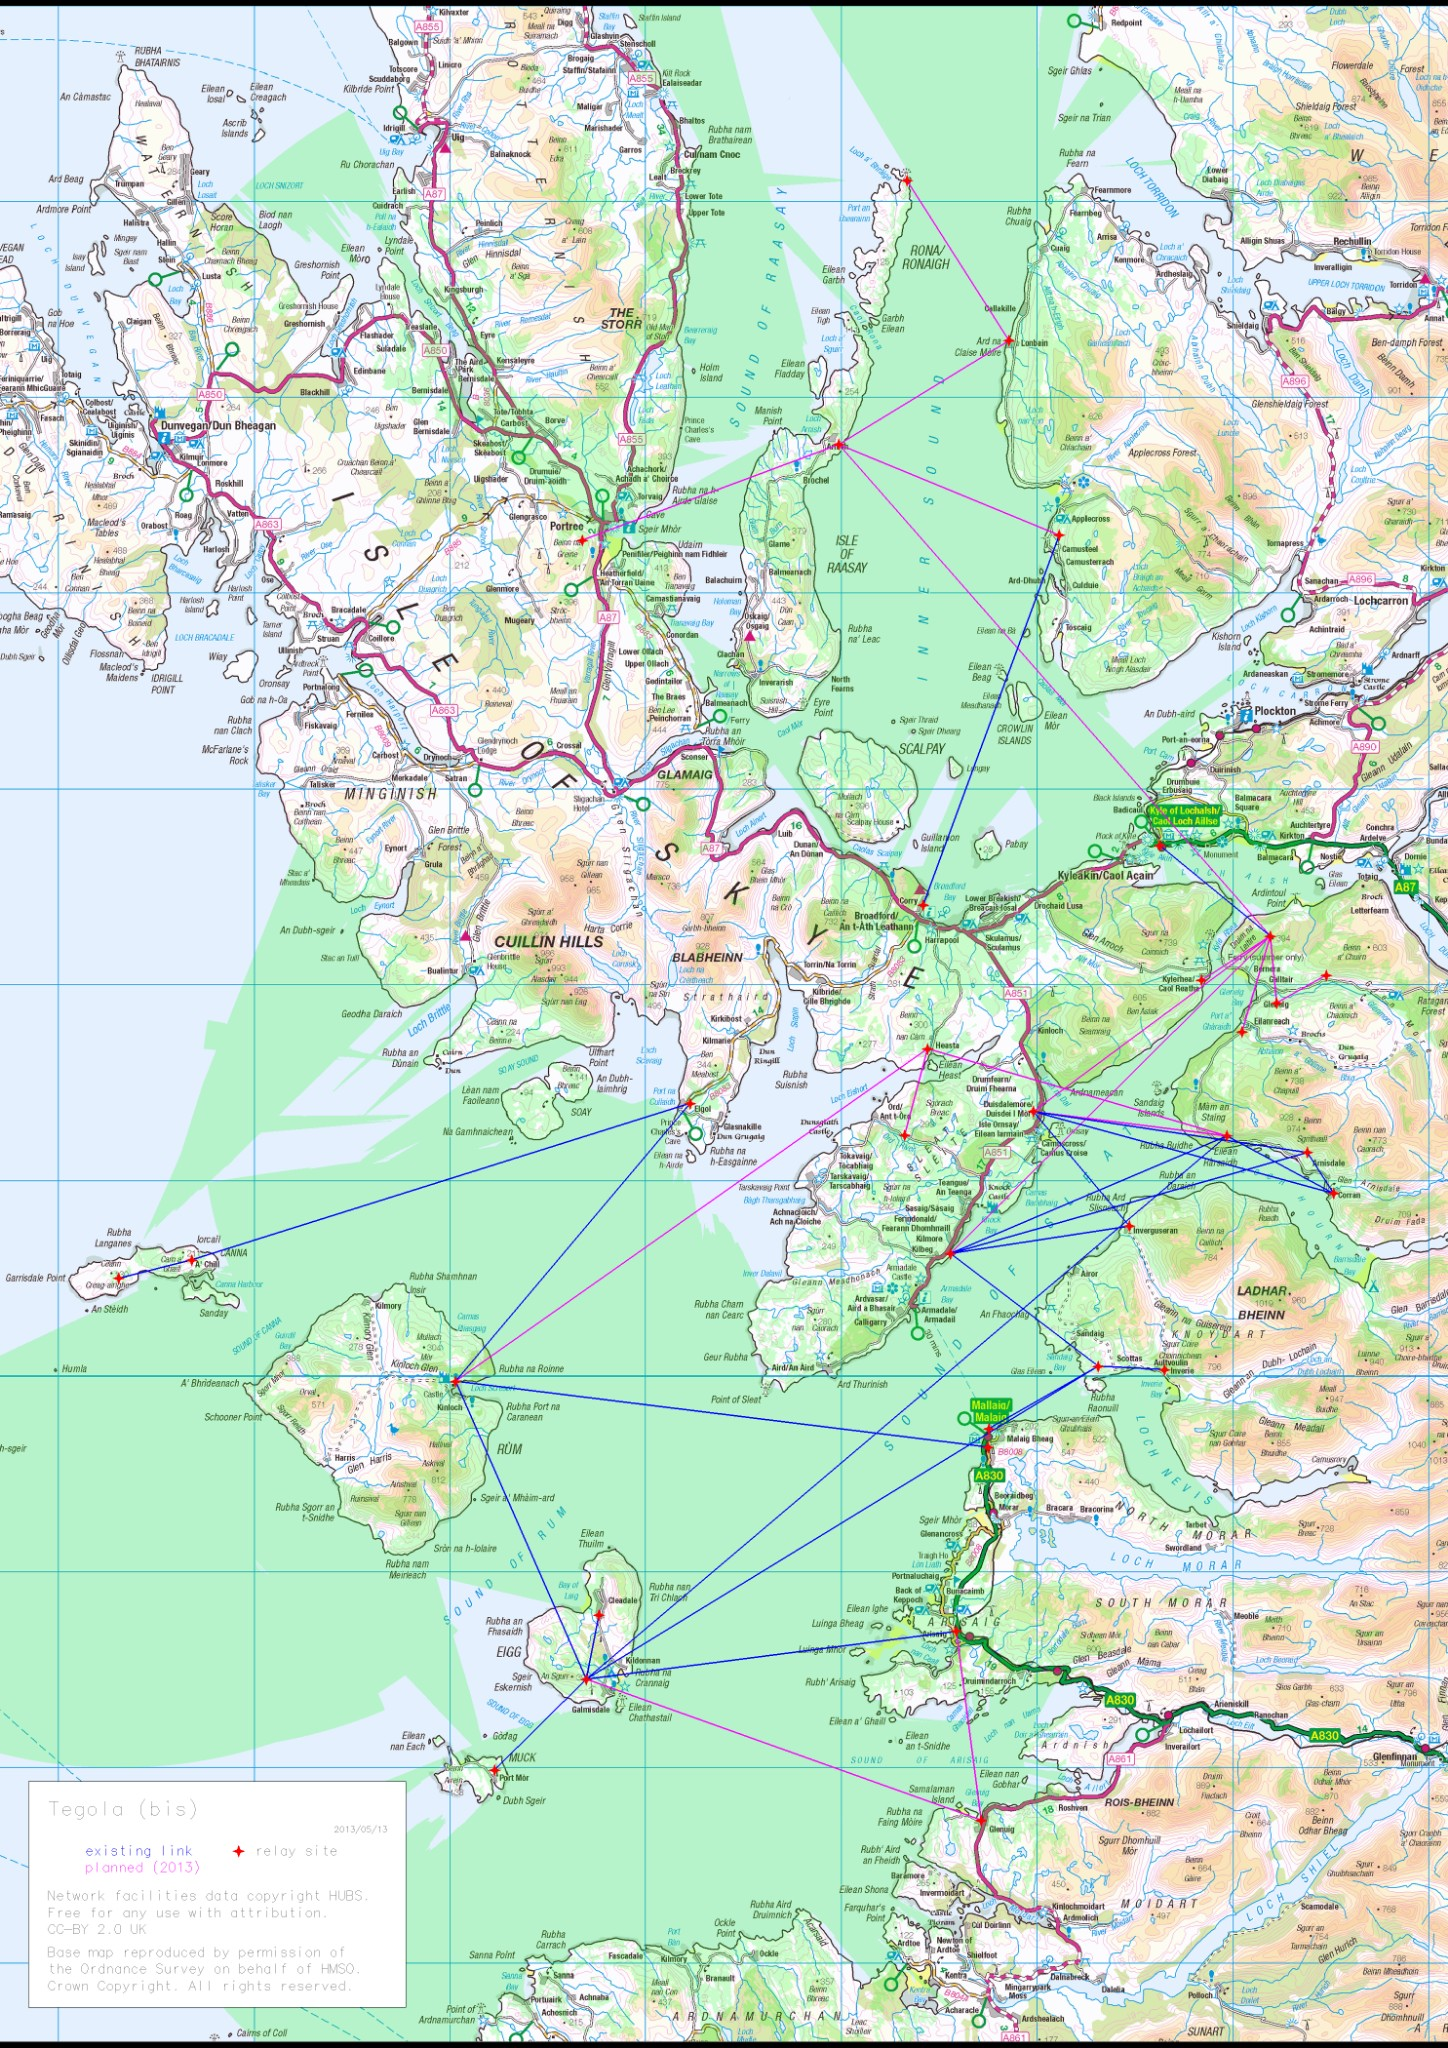
\includegraphics[width=\textwidth]{west_coast_a4.jpg}};
          \end{scope}
        \end{tikzpicture}
      }
    \end{center}
    \column{0.7\textwidth}
    \begin{itemize}
      \item Connect adjacent networks
      \item Inter-community backbone with BGP
      \item Cheap radios only as bridges
      \item FreeBSD + bird, or Mikrotik
      \item Let individual networks be
      \item Redundant paths are good
        \begin{itemize}
          \item Fibre cut in Lochcarron takes out all BT services, our
            network stays up
          \item Power cut takes out Sabhal M\`{o}r Ostaig over the
            Christmas Holidays
          \item Lightening strike melts phone lines, NHS uses
            community network
        \end{itemize}
    \end{itemize}
  \end{columns}
\end{frame}
\begin{frame}{HUBS: Formalising the model}
  \begin{columns}
    \column{0.4\textwidth}
    \includegraphics[width=\textwidth]{confederation.eps}\\
    \vspace{-0.5\baselineskip}
    \begin{center}
      
\includegraphics[height=0.07\textheight]{UHI_Logo_CMYK}
      \hspace{1pt}
      \includegraphics[height=0.07\textheight]{eushield-fullcolour}
      \hspace{1pt}
      \includegraphics[height=0.07\textheight]{smo-pms-blue}\\
      \vspace{0.25\baselineskip}
%      \hspace{1pt}
      
\includegraphics[height=0.07\textheight]{stir-logo-colour}
      \hspace{1pt}
      \includegraphics[height=0.07\textheight]{carnegie-logo.jpg}
      \hspace{1pt}
      
\includegraphics[height=0.07\textheight]{leader-and-words.jpg}
      \hspace{1pt}
      \includegraphics[height=0.07\textheight]{eu-and-words.jpg}\\
      \begin{tikzpicture}[overlay]
          \node at (0, 0.1) {%
            
\includegraphics[height=0.125\textheight]{Fluency_2013_logo.pdf}
          };
      \end{tikzpicture}
    \end{center}
    \column{0.6\textwidth}
    \begin{itemize}
      \item Each community network encapsulated in an autonomous
        system
      \item Retain diverse internal structures according to what the
        operators are comfortable with
      \item Collective negotiation of transit, carrier services
      \item Seen by the outside world as a BGP confederation behind
        AS60241
      \item Currently two confederations, the West Coast and
        South Scotland
    \end{itemize}
  \end{columns}
\end{frame}
\begin{frame}{The HUBS Network (South)}
  \begin{center}
    \includegraphics[width=0.9\textwidth]{hubs-nov2014.eps}
  \end{center}
\end{frame}
\begin{frame}{Impact}
  \begin{tikzpicture}
    \begin{scope}
      \clip (-5,-1.5) rectangle (6,1.5);
      \node at (0,0) {
        \includegraphics[width=\textwidth]{mhialairigh-doctored1.png}
      };
    \end{scope}
  \end{tikzpicture}
  \begin{itemize}
    \item Distance learning for adults (e.g. UHI)
    \item Distance learning for children (e.g. GLOW $=$ Scottish
      schools national intranet)\\
      $\rightarrow$ Children on Eigg schooling even in bad weather.
    \item Local businesses no longer disadvantaged\\
      $\ldots$ have even seen \textit{new} ones moving in!
    \item Telemedicine starts to be practised
  \end{itemize}
  \hfill$\ldots$\textit{Symmetry is appreciated}
\end{frame}
\begin{frame}{Layer $\leq$ 7}
  \begin{columns}
    \column{0.5\textwidth}
    \includegraphics[width=\textwidth]{creagan-dearga-mast.jpg}\\
    \begin{itemize}
      \item Slow IPv6 adoption
      \item Variable equipment quality
      \item Outgrowing available capacity on the West
        Coast
    \end{itemize}
    \column{0.56\textwidth}
    \begin{itemize}
      \item Heavy use of NAT breaks picocells trying to do IPSec
      \item Heavy use of NAT can lead Google to accuse community
        networks of having worms\\
        $\ldots$ Similar to anonymity networks like \texttt{tor}
      \item RFC1918 address collisions between UHI and the community
        networks cause pain
      \item Use of ADSL lines is \textit{extremely} expensive (cf.
        BT WBC tarrif) and providers notice
    \end{itemize}
  \end{columns}
\end{frame}
\begin{frame}
  \frametitle{Layer $\geq$ 8}
  \begin{columns}
    \column{0.6\textwidth}
    \begin{itemize}
      \item Step-Change, BDUK and ScotGov / CBS funding
        \begin{itemize}
          \item Cumbersome process
          \item State Aid \& Double Funding
          \item Little in-house expertise
        \end{itemize}
      \item BT's network build
        \begin{itemize}
          \item An\ae{}mic Open Access
          \item Opaque process
          \item Territorial ``disputes''
        \end{itemize}
      \item Education -- not vendor courses, not ``enterprise''
        courses, but ``West Highland Engineering''
      \item \textbf{\color{hubsblue} Summer School Next Year --
        Volunteers to visit \& teach?}
    \end{itemize}
    \column{0.4\textwidth}
    \hspace{-2em}\includegraphics[width=1.1\textwidth]{portree-3d.png}\\
    \hspace{-2em}\includegraphics[width=0.55\textwidth]{HIE-NGA-Deployment-2013-10-25.pdf}
    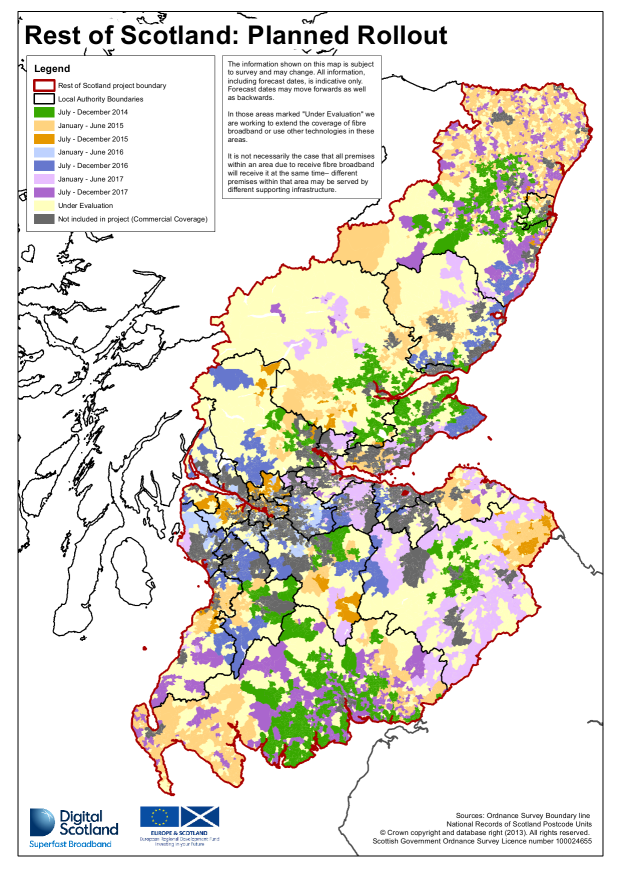
\includegraphics[width=0.55\textwidth]{ros.png}
  \end{columns}
\end{frame}
\begin{frame}
  \begin{center}
    \begin{tikzpicture}[overlay]
      \node at (0, -0.5) {%
        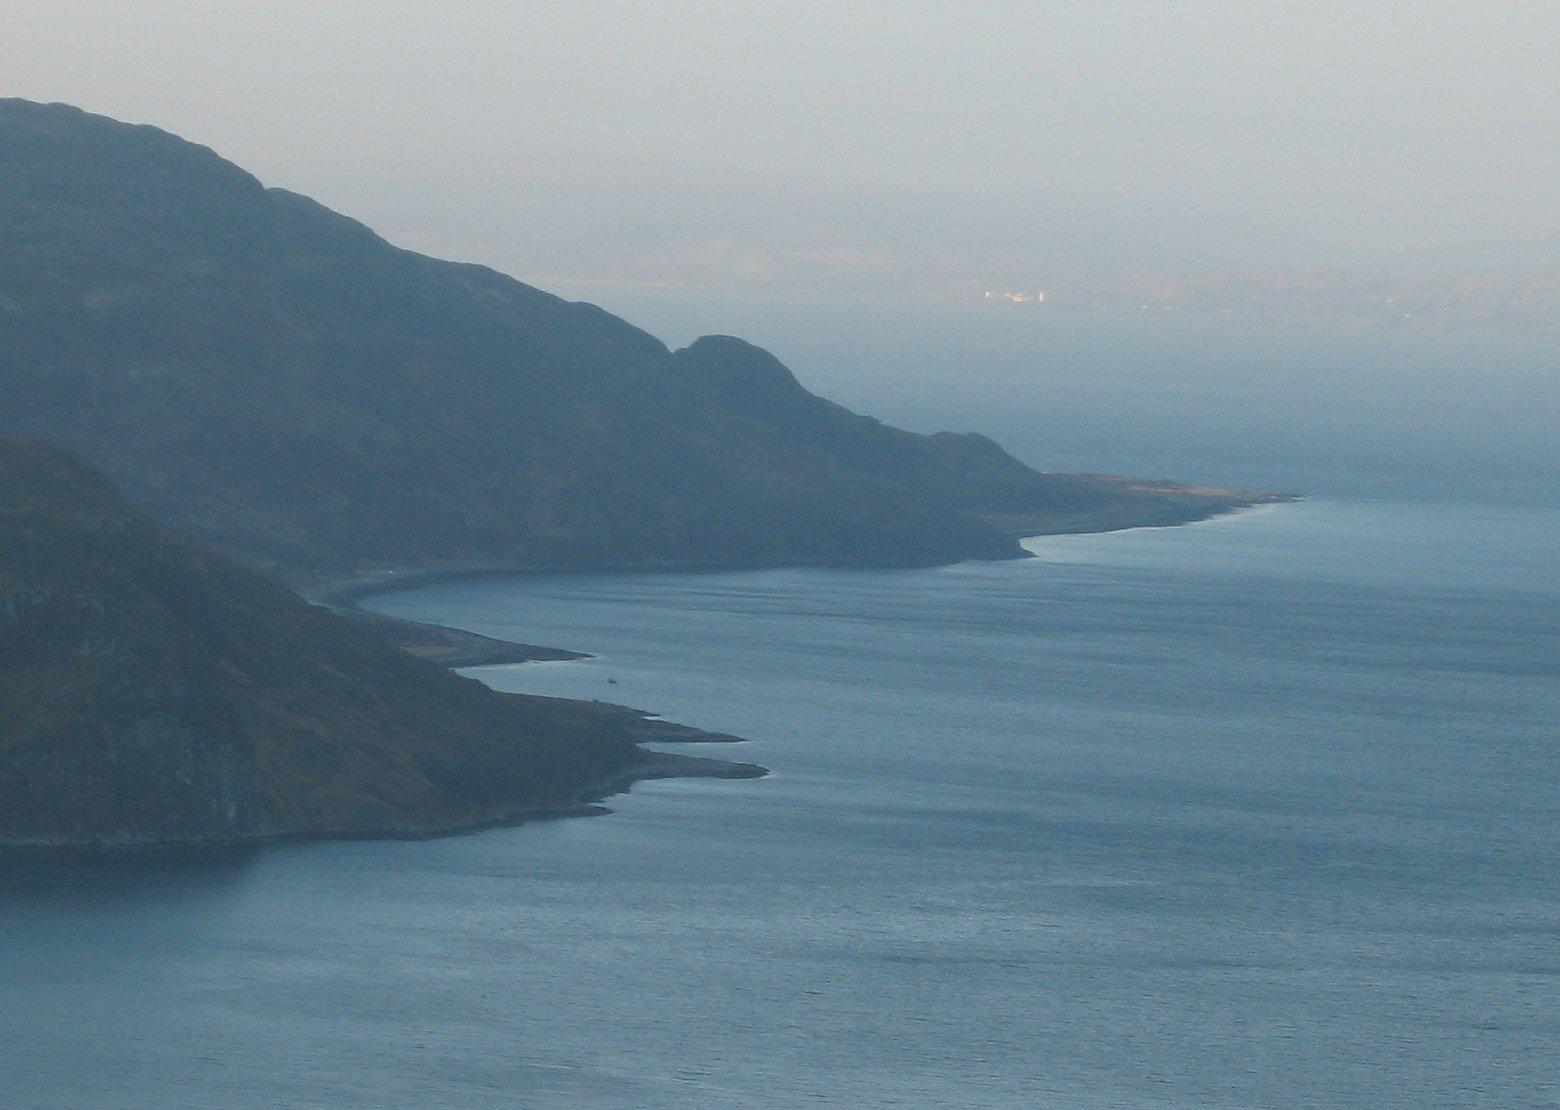
\includegraphics[height=1.1\paperheight]{scenery.jpg}
      };%
      \node at (4,3) {\Huge \color{hubsblue} Thank you};
      \node at (0,-4) {\Large \color{hubsblue}\url{http://www.tegola.org.uk/}};
      \node at (0,-4.5) {\Large \color{hubsblue}\url{http://www.hubs.net.uk/}};
    \end{tikzpicture}
  \end{center}
\end{frame}    

\end{document}
